\documentclass{article}

\usepackage{graphicx}
\usepackage{subfig}
\usepackage[hidelinks]{hyperref}

\begin{document}
    \begin{titlepage}
        \centering
        {\bfseries\LARGE Universidad Rey Juan Carlos\par}
        \vspace{1cm}
        {\scshape\Large Ingenier\'ia de Rob\'otica Software \par}
        \vspace{3cm}
        {\scshape\Huge Rob\'otica aerea \par}
        \vspace{3cm}
        {\itshape\Large Problema 1 Tema 3 \par}
        \vfill
        {\Large Autor: \par}
        {\Large Daniel Alejandro Quinga L\'opez \par}
        \vfill
        {\Large Octubre 2023 \par}
    \end{titlepage}

    \newpage
    
    La aeronave de ala fija a estudiar es el \href{https://en.wikipedia.org/wiki/Bombardier_Global_7500}{\textbf{Bombardier Global 7500}}.
    \begin{figure}[h]
        \centerline{\hspace{0cm}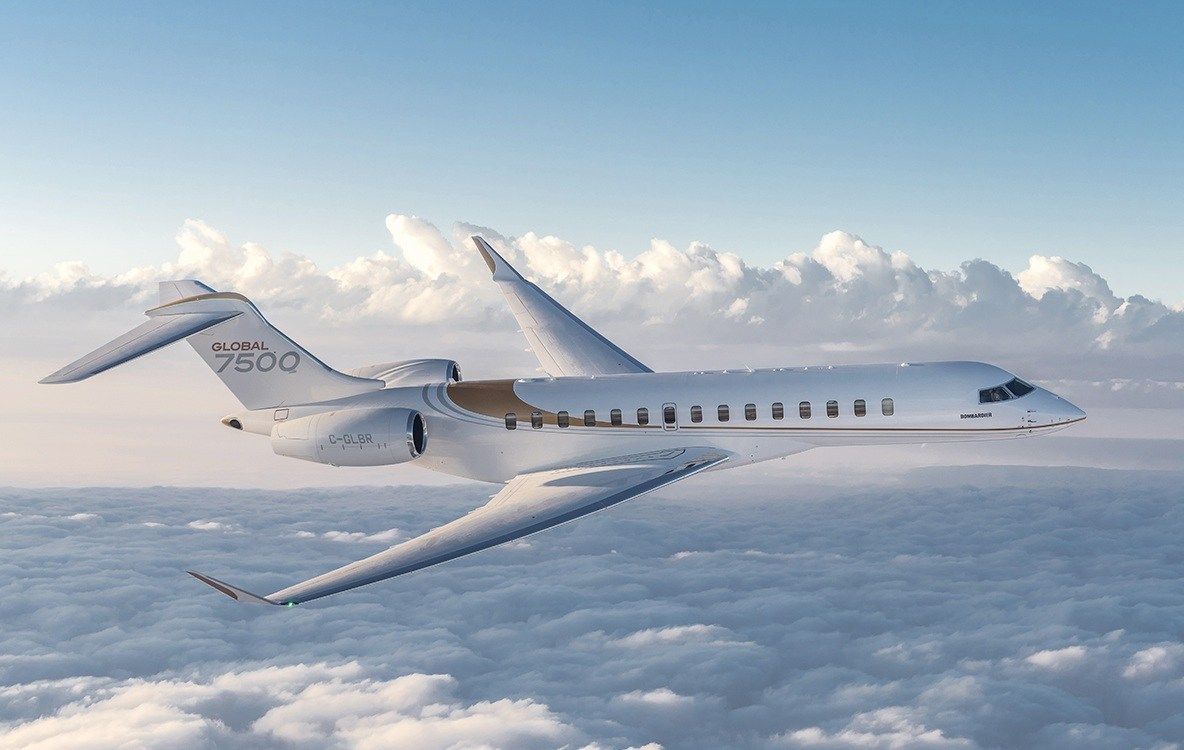
\includegraphics[width=0.66\columnwidth]{BombardierGlobal.jpg}}
        \caption{Bombardier Global 7500.}\label{fig:figura_1}
    \end{figure}


    Su altitud de vuelo de crucero: 51,000 pies (15,545 metros).
    \newline
    Su velocidad de vuelo de crucero: Mach 0.85 (487 kt / 902 km/h / 250.56 m/s).
    \newline
    Su peso máximo de despegue (MTOW): Alrededor de 114,850 libras (52,096 kg).
    \newline

    \begin{enumerate}
        \item ¿Cuál es la sustentación necesaria?
        
        \bigskip
        La \textbf{sustentaci\'on} es la fuerza aerodinámica que actúa sobre una aeronave y la mantiene en el aire.
        \begin{center}
            $L = C_{L} \cdot \frac{1}{2} \cdot \rho \cdot S \cdot V^2$.
        \end{center}

        Para un vuelo horizontal a velocidad constante, la fuerza de sustentación tiene que ser igual al peso de la aeronave.
        \begin{center}
            $L = W = m \cdot g = 52096 \cdot 9.8 = 510540.8 N$
        \end{center}
        
        \item Seleccionar un perfil en http://airfoiltools.com que nos permita volar en estas
        condiciones sin entrar en pérdida y con Momentos respecto al centro aerodinámico
        cercano a 0.

        \bigskip
        Con los datos de sustentación del apartado anterior, calculamos el $C_{L}$ necesario para mantener el vuelo horizontal.
        \newline
        Para ello primero se debe calcular la densidad del aire a 15,545 metros.
        \begin{center}
            $T = T_{o} - 6.5 \cdot \frac{h}{1000} = 288.15 - 6.5 \cdot \frac{15545}{1000} = 186.91K$
        
            $p = p_{o}(1 - 0.0065(\frac{h}{T_{o}}))^{5,2561} = 1.012 \cdot 10^5(1 - 0.0065(\frac{15545}{288.15}))^{5,2561} = 10459.661Pa$
            
            $\rho = \frac{p}{RT} = \frac{10459.661}{287 \cdot 186.91} = 0.195 kg/m^3$
        \end{center}
        Ahora se calcula el $C_{L}$ sabiendo que la superficie alar del avión es 116.5 $m^2$.
        \begin{center}
            $C_{L} = \frac{L}{\frac{1}{2} \cdot \rho \cdot S \cdot V^2} = \frac{510540.8}{\frac{1}{2} \cdot 0.195 \cdot 116.5 \cdot 250.56^2} = 0.6623$
        \end{center}

        Ahora seleccionamos en la web airfoiltools.com un perfil aerodinámico que nos
        permita ese $C_{L}$ y que al mismo ángulo de ataque tenga un $C_{MCA}$ similar a 0.

        Para saber qué curva tenemos que mirar calculamos el número de Reynolds aproximado (aproximamos la cuerda como 5.825 m para un avión con S = 116.5 $m^2$):
        
        \begin{center}
            $Re = \frac{\rho V L}{\mu} = \frac{0.195 \cdot 250.26 \cdot 5.825}{1,8 \cdot 10^-5} = 15811380$
        \end{center}
        Miramos el Re de 1 millón (a partir de ese número las curvas ya no cambian mucho).
        \newline
        
        \begin{figure}[h]
            \centering
             \subfloat[CLvsALPHA]{\label{f:figura_2}
               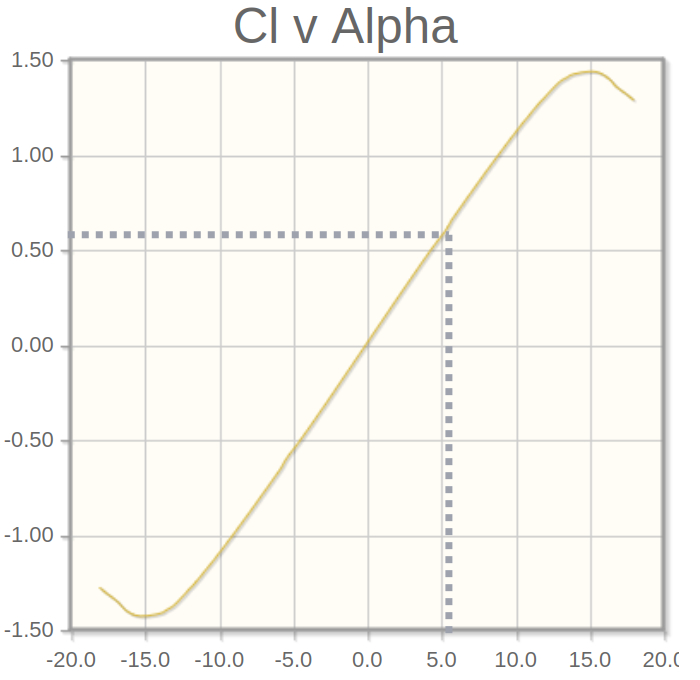
\includegraphics[width=0.44\columnwidth]{CLvsALPHA.jpg}}
             \subfloat[CLvsALPHA]{\label{f:figura_3}
               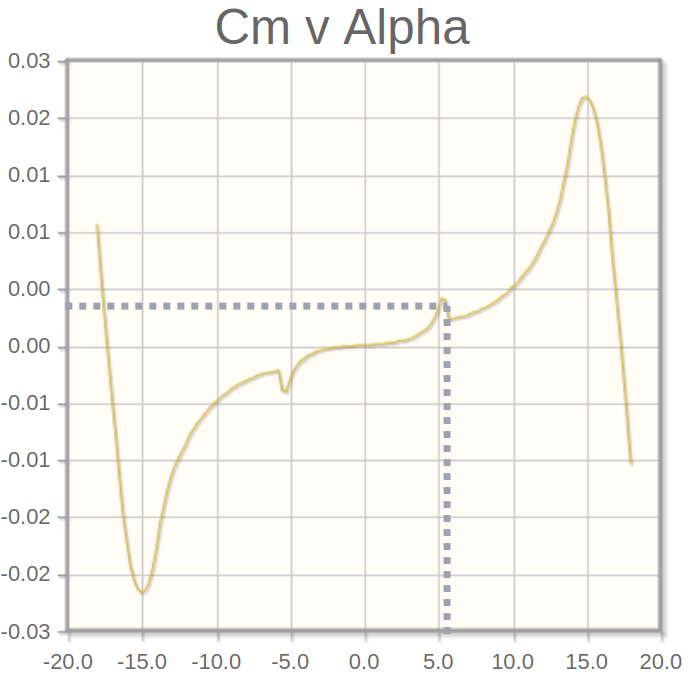
\includegraphics[width=0.44\columnwidth]{CMvALPHA.jpg}}
            \caption{CL v ALPHA y CM v ALPHA}\label{f:graphics}
        \end{figure}
        Un perfil que cumple con los requisitos es \href{http://airfoiltools.com/airfoil/details?airfoil=joukowsk-il}{12\% JOUKOWSKI AIRFOIL \- 12\% Joukowski airfoil}.
        \newline
        Observando las gráficas podemos apreciar que el ángulo de ataque es aproximadamente 6º.

        \item Determinar la fuerza de resistencia aerodinámica que ejercerá el ala.
        
        \bigskip

        El coeficiente de resistencia se obtiene a partir del perfil seleccionado siendo aproximadamente 0.009.
        \newline
        \begin{figure}
            \centering
                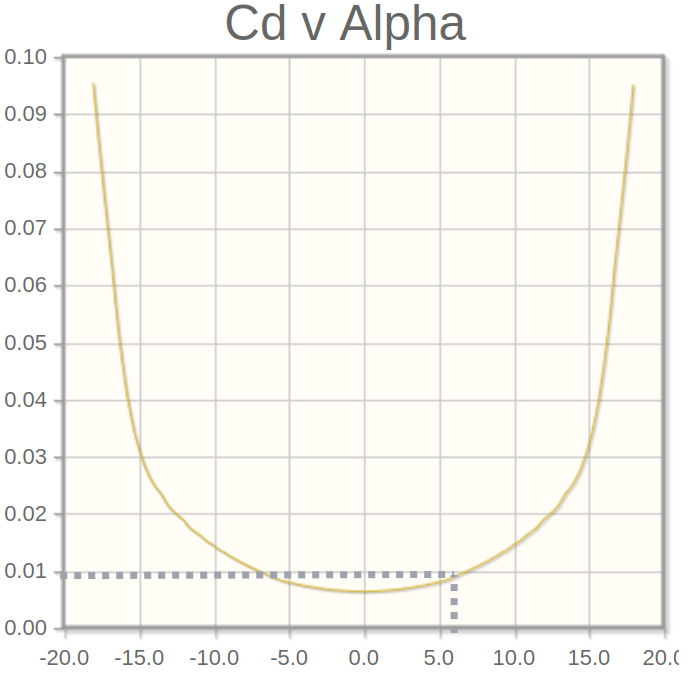
\includegraphics[width=0.44\columnwidth]{CdvAlpha.jpg}
            \caption{Cd v Alpha.}\label{fig:figura_4}
        \end{figure}
        \newline
        
        Por último para el cálculo de la fuerza de resistencia aerodinámica se aplica la siguiente fórmula.
        \begin{center}
            $D = C_{D} \cdot \frac{1}{2} \cdot \rho S V^2 = 0.009 \cdot \frac{1}{2} \cdot 0.195 \cdot 116.5 \cdot 250.56^2 = 6402,59N$
        \end{center}

    \end{enumerate} 

\end{document} 